\documentclass[a4paper, 12pt]{article}%тип документа

%отступы
\usepackage[left=2cm,right=2cm,top=2cm,bottom=3cm,bindingoffset=0cm]{geometry}

%Русский язык
\usepackage[T2A]{fontenc} %кодировка
\usepackage{gensymb}
\usepackage[utf8]{inputenc} %кодировка исходного кода
\usepackage[english,russian]{babel} %локализация и переносы

%Вставка картинок
\usepackage{wrapfig}
\usepackage{graphicx}
\graphicspath{{pictures/}}
\DeclareGraphicsExtensions{.pdf,.png,.jpg}

%Графики
\usepackage{multirow}
\usepackage{pgfplots}
\pgfplotsset{compat=1.9}

%Математика
\usepackage{amsmath, amsfonts, amssymb, amsthm, mathtools}

%Заголовок
\author{Сифат Мд Абдуллах Ал Хасиб \\
Физтех школа электроники, фотоники и молекулярной физики \\
Группа Б04-105}
\title{\textbf{Лаборатория Работа 3 \\ 
Определение энтальпии реакции нейтрализации сильной кислоты сильным основанием}}
\begin{document}
\maketitle
\section{Введение}\textbf{Цель работы:} Определить энтальпию реакции нейтрализации соляной кислоты гидроксидом калия.\\
\textbf{В работе используется:} Калориметр, термометр, магнитная мешалка, соляная кислота, гидроксид калия. 
\section{Теоретическая справка}
Из первого закона термодинамики мы знаем, что\\
\begin{center}
$ Q_p = \Delta U+ P\Delta V$                     (1)
\end{center}
Где $\Delta U$ - внутренняя энергия, $P$ - давление, $\Delta V$ - изменение объема, а $Q_p$ - тепло. При изохорном процессе (V = const) поглощение или выделение тепла (тепловой эффект) связано только с изменением внутренней энергии:\\
\begin{center}
$Q_v = \Delta U$
\end{center}
В химии чаще всего рассматривают изобарные процессы (Р = const), и тепловой эффект в этом случае называют изменением энтальпии системы или энтальпией процесса:
\begin{center}
$|Q_p| = |\Delta H|$,\\
$\Delta H = \Delta U + P\Delta V.$
\end{center}
Энтальпия имеет размерность энергии (кДж). Её величина пропорциональна количеству вещества; энтальпия единицы количества вещества (моль) измеряется в $ \text{кДж.моль}^\text{-1}$.\\
\newpage В термодинамической системе выделяющуюся теплоту химического процесса условились считать отрицательной (экзотермический процесс, $\Delta Н < 0$), а поглощение системой теплоты соответствует эндотермическому процессу, $\Delta Н > 0$. Энтальпия, как и остальные термодинамические функции, для удобства сопоставления отнесена к некоему стандартному состоянию веществ (Т = 298 К, Р = 101325 Па, единице количества вещества). В этих условиях изменение термодинамических функций обозначают нижним индексом 298, и верхним  индексом 0 ($ \Delta H^0_{298}$). Обычно нижний индекс не указывают, тогда стандартные значения энтальпии $ \Delta H^0$.\\
\linebreak В экзотермической реакции нейтрализации сильной кислоты сильным основанием энтальпия (выделившееся тепло) пропорциональна количеству вещества:
\[\Delta H = n \Delta H^0, \text{к.Дж}  (2)\]
где n – количество вещества (протонов), участвующих в реакции, моль\\ Это тепло расходуется на нагревание реакционной смеси и сосуда:
\[Q = K\dot{•}\Delta t, \text{к.Дж} (3)\] 
$\Delta t = t_{\text{кон}} - t_{\text{нач}}$ -  повышение температуры системы, $\degree C$. \\
\linebreak Коэффициент пропорциональности К в (3)  равен суммарной теплоемкости сосуда и раствора и носит название тепловой постоянной калориметра. Объединив формулы (2) и (3) можно рассчитать стандартную энтальпию реакции:
\[n\Delta H^0 = -K \Delta t \rightarrow \Delta H = \frac{K \Delta H}{n•}\]

Чтобы устранить искажение истинной величины $\Delta T$ в результате частичных потерь тепла в окружающую среду, используют графический метод ее определения. С этой целью записывают изменение температуры в зависимости от времени до начала химического процесса (предварительный период), во время его течения (главный период) и после его окончания (заключительный период). Характерная кривая приведена на рис 1.
\begin{figure}
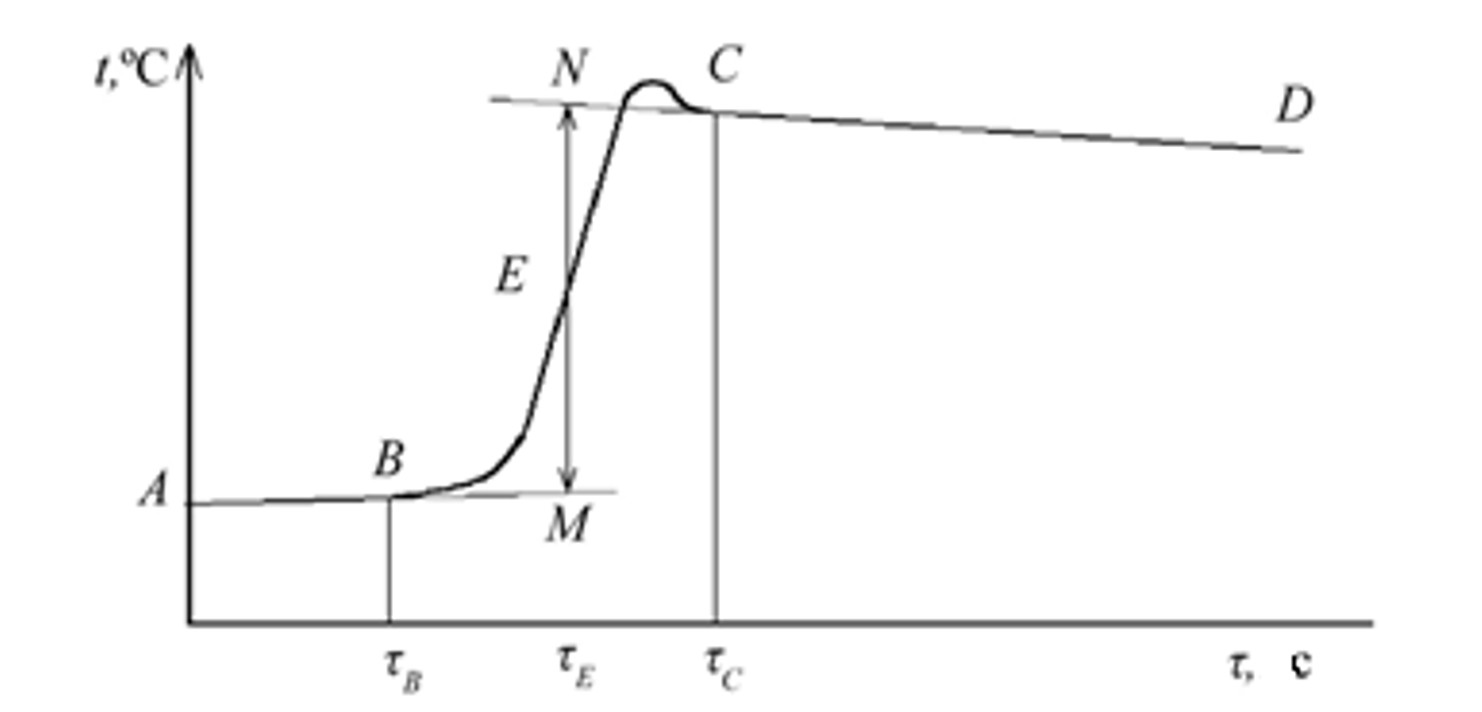
\includegraphics[width = 0.9\textwidth]{fig1.png}
\caption{ Изменение температуры в зависимости от времени для экзотермического процесса}
\end{figure}

Момент окончания химического процесса $ \tau c$ определяют по установлению плавного монотонного хода кривой $ t(\tau)$. Находят середину главного периода $\tau E$, восстанавливают из точки $\tau E$ перпендикуляр и экстраполируют кривые АВ и СD до пересечения с этим перпендикуляром в точках М и N. Истинное изменение температуры равно отрезку МN.

\section{Экспериментальная установка}
Экспериментально энтальпия химических реакций определяется изменением температуры реакционной смеси во время реакции при соблюдении определенных условий, ограничивающих энергообмен с окружающей средой. Обычно для этой цели используются специальные калориметры. Внешний вид калориметра показан на рис.2. Мы включили магнитную мешалку, налили 115 мл гидроксида калия в коническую колбу и поместили ее внутрь калориметра. Затем мы снова взяли 100 мл соляной кислоты и тоже отнесли ее в калориметр. Поскольку мы провели реакцию между основным гидроксидом калия и соляной кислотой, температура реакции изменится, как показано на термометре
\begin{figure}
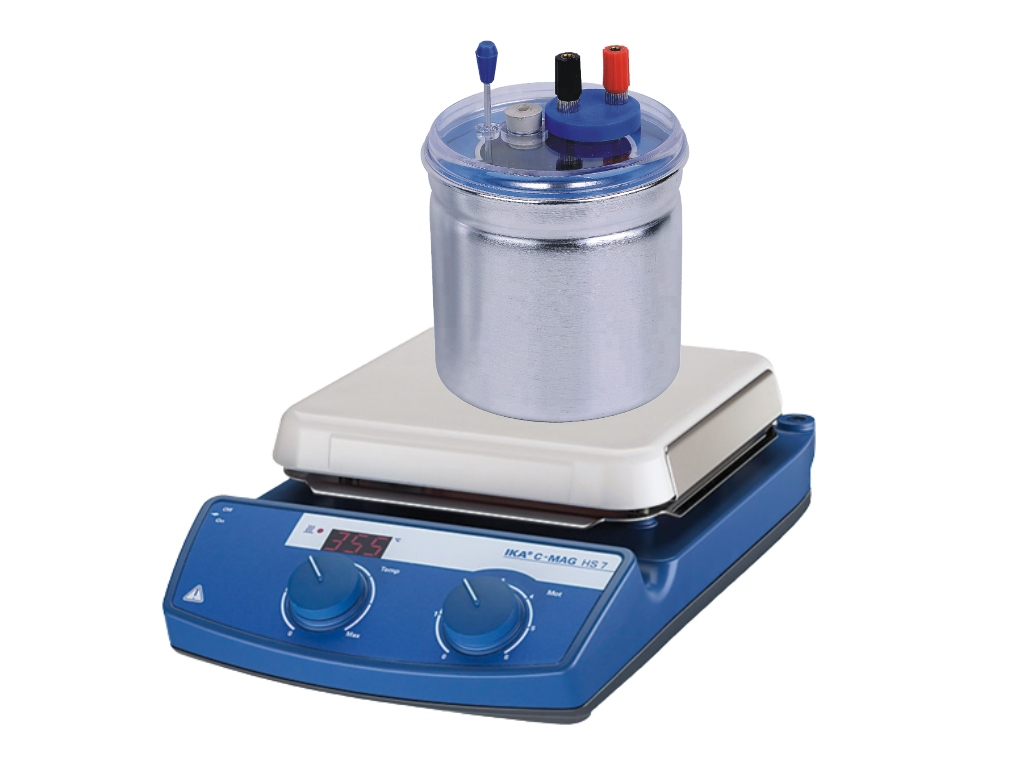
\includegraphics[width = 0.9\textwidth]{fig2.jpg}
\caption{Схема установки}
\end{figure}
\newpage{}
\section{Ход работы}
После того, как мы отмерили в один цилиндр 110 мл 1 H раствора КОН, а во второй – 100 мл 1 Н раствора HCl – сильной кислоты, опускаем в калориметр магнит, заливаем в него 110 мл щелочи, закрываем крышку и ставим его на магнитную мешалку. Включив мешалку, в течение 2–3 мин через каждые 10 секунд записываем температуру раствора в предварительном периоде с точностью 0,05 \degree C. В течение всего времени замера она оставалась неизменной и составила: 
\[t_A = 22.3 \degree C\]
В момент очередного отсчета начнём аккуратно и медленно по стеклянной палочке вливать в калориметр через воронку кислоту. С начала и до конца вливания, показания термометра записываем и заносим в таблицу.

\begin{table}[h!]
\centering
\begin{tabular}{|c|c|c|c|c|c|c|c|c|c|c|c|c|}
\hline
$\tau_0 - \tau_B$, ceк & 0,00 & 1,00 & 2,16 & 7,30 & 11,6 & 15,50 & 20,80 & 24,12 & 27,33 & 31,50 & 35,17 & 41,25  \\ \hline
t, \degree C & 22,3 & 23,0 & 24,0 & 25,0 & 26,0 & 27,0 & 28,0 & 29,0 & 30,0 & 31,0 & 32,0 & 31,0 \\ \hline

\end{tabular}
\caption{Зависимость температуры содержимого от времени}
\label{tab:second_tube_parametrs}
\end{table}
Максимальная температура была 32 \degree C, а после этого, как видно из данных, элементы калориметра начали охлаждаться, и температура снизилась до 31 \degree C. Таким образом, середине процесса соответствует координата:
\begin{center}
$\tau_E - \tau_B = 20,63$ сек

\end{center} 
Моментом начала заключительного периода можно считать момент времени
\begin{center}
$\tau_C - \tau_B = 41,25$ сек
\end{center} 
За последующие 8,5 минут температура содержимого остыла ровно на 0,5 \degree C.
\begin{center}
$\tau_D \approx 406$ сек

\end{center} 
Используя полученные данные, мы построили график зависимости температуры от времени и показали его на рис. 3:\\ 


\begin{figure}[h]
\center
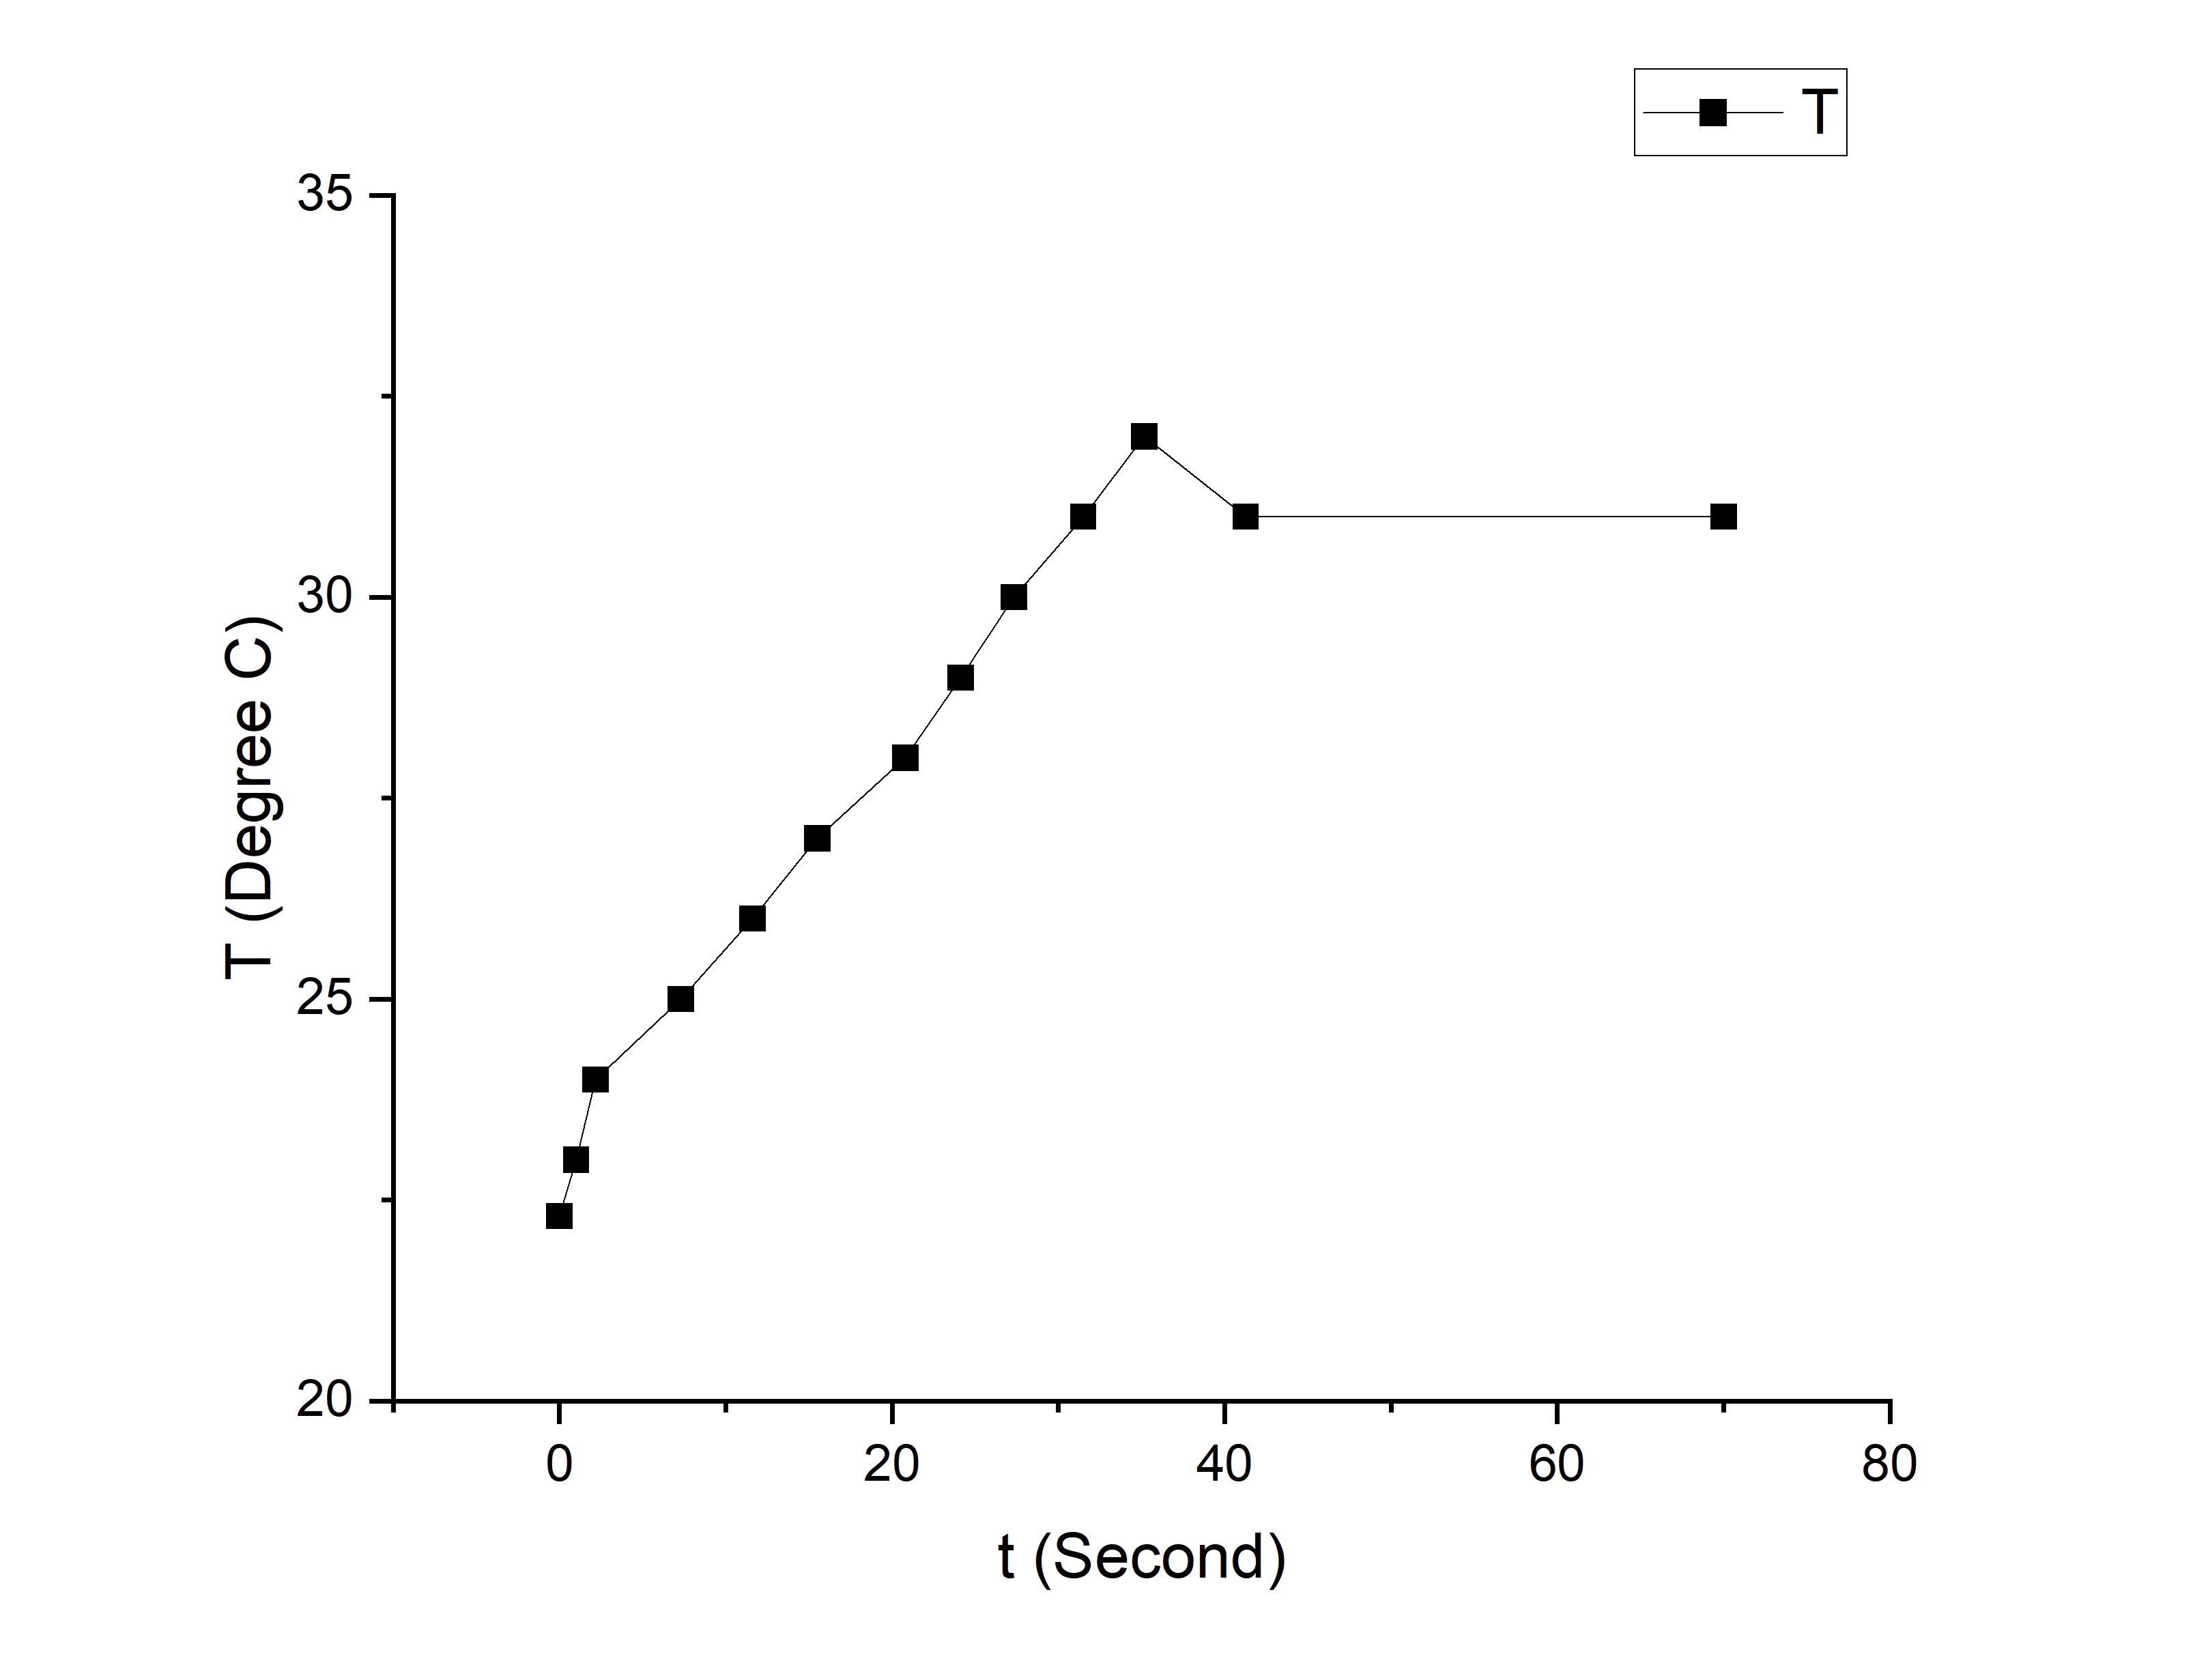
\includegraphics[scale=0.5]{labphoto13.png}
\caption{ График температуры в зависимости от времени.}
\end{figure}

 Графически определим $\Delta t$:
\begin{center}
$\Delta t = 8,7 \degree C$
\end{center}
Теплоту нейтрализации можно определить по следующей формуле:
\begin{center}
$ \Delta H_{\text {нейтр}} = \frac{K \Delta t}{V C_H}$
\end{center}
где $C_H$ – нормальность кислоты (в нашем случае 1 моль.л-1), V – её объём, K – постоянная калориметра (в нашем случае 0,76). 
Таким образом:
\begin{center}
$ \Delta H_{\text {нейтр}} = -66,2$  $\text{кДж.моль}^\text{-1}$
\end{center}
\newpage
\section{Вывод}
Реакция, произошедшая в нашем эксперименте, была
\begin{center}
$HCl + KOH \rightarrow KCl + H_2O$
\end{center}
Из эксперимента мы получили значение энтальпии $ \Delta H_{\text {нейтр}} = -66,2$  $\text{кДж.моль}^\text{-1}$. Мы видим, что заданное значение таблицы $ \Delta H_{\text {нейтр табл}} = -55,9$  $\text{кДж.моль}^\text{-1}$. Наше экспериментальное значение немного отличается от табличного. Стоит учитывать, что точность полученного значения зависит от человеческих факторов, что может быть главной причиной такого отклонения. Объяснить понижение температуры или же “горбик” можно неравномерным распределением температуры: у места, куда мы вливаем, температура выше, поэтому при перемешивании температура потом уменьшается.  



\end{document}